\documentclass[11pt, a4paper, landscape]{article}
\usepackage[american, userlastpage, triangle, vertical,utf-8]{NeyDreuwSlides_Oct08}
\usepackage{multimedia}

\renewcommand*{\title}{Deep Directed Generative Models}                               % main title of the work (used for \TitlePage)
\renewcommand*{\titleshort}{Generative Models}                    % short title (used for \lfoot)
\renewcommand*{\occasion}{Seminar Selected Topics in WS 2016/2017--} % (used for \TitlePage)
\renewcommand*{\occasionshort}{Selected Topics WS 2016/2017}  % short occasion title (used for \rfoot)
\renewcommand*{\date}{01.02.2017}
\renewcommand*{\author}{André Merboldt}                                     % all the authors of the work, can be long (used for \TitlePage)
\renewcommand*{\authorshort}{Merboldt, }                                        % all the authors of the work, should be short (used for \lfoot)
\renewcommand*{\email}{\url{andre.merboldt@rwth-aachen.de}}             % all email address(es) of the authors (used for \TitlePage)
\renewcommand*{\mainauthor}{André Merboldt}                                 % the author(s) who presented the work (used for \FinalPage)
\renewcommand*{\mainauthoremail}{\email}                                  % presenter mail address(es) (used for \FinalPage)
\renewcommand*{\www}{http://www-i6.informatik.rwth-aachen.de/}            % web address (used for \TitlePage _and_ \FinalPage)
\newcommand*{\keywords}{Generative Models, Deep Learning, Generative Adversarial Network, Variational autoencoder, sigmoid belief net, variational inference, reparameterization trick}      % keywords for pdf summary


% will be set into the PDF document summary
\hypersetup{
  pdftitle={\title}, 
  pdfsubject={\occasion},  
  pdfauthor={\author}, 
  pdfkeywords={\keywords}
}


\begin{document}

%%%%%%%%%%%%%%%%%%%%%%%%%%%%%%%%%%%%%%%%%%%%%%%%%
\TitlePage


%%%%%%%%%%%%%%%%%%%%%%%%%%%%%%%%%%%%%%%%%%%%%%%%%
\NewPage\headline{Outline}
\vfill
\begin{itemize}
\item[] \hyperlink{sli:introduction}{Introduction}
  \item[] \hyperlink{sli:sbn}{Sigmoid Belief Nets}
  \item[] \hyperlink{sli:vae}{Variational Autoencoders}
  \item[] \hyperlink{sli:gan}{Generative Adversarial Nets}
  \item[] \hyperlink{sli:more}{More Generative Models}
\item[] \hyperlink{sli:summary}{Summary}
\item[] \hyperlink{sli:references}{References}
%\item[] \hyperlink{sli:results}{Results}
\end{itemize}
\vfill


%%%%%%%%%%%%%%%%%%%%%%%%%%%%%%%%%%%%%%%%%%%%%%%%%
\NewPage\headline{Introduction}
\hypertarget{sli:introduction}
\vfill
\begin{itemize}
  \item Challenging task
  \begin{itemize}
    \item Complex and expressive
    \item Scalable and tractable
  \end{itemize}
\end{itemize}
...
\vfill

%%%%%%%%%%%%%%%%%%%%%%%%%%%%%%%%%%%%%%%%%%%%%%%%%
\NewPage\headline{Why Generative Models: Applications}
\hypertarget{sli:why}
\vfill
\begin{itemize}
  \item Unsupervised learning
  \item Understand data better (Dimensionality reduction)
  \item Representation learning
  \item Generative image modelling
  \begin{itemize}
    \item Compression
    \item Super-resolution
    \item Denoising
  \end{itemize}
  \item ... Generate data
\end{itemize}
\vfill


%%%%%%%%%%%%%%%%%%%%%%%%%%%%%%%%%%%%%%%%%%%%%%%%%
\NewPage\headline{Deep Directed Graphical Model}
\hypertarget{sli:formal}
\vfill
\begin{itemize}
  %\item Dataset $X = (x^{(1)}, x^{(2)}, \dots, x^{(n)})$
  \item Data generation process is $x \sim p(x)$
  \item We assume that $x$ depends on hidden variable $z$:
  \begin{itemize}
    \item $z \sim p(z)$ and $x \sim p(x|z)$
  \end{itemize}
  \item Our goal is to generate more $x$ by sampling from $p(x)$
  \item However: $p(x) = \sum_{z} p(x|z) p(z)$
  \begin{itemize}
    \item Intractable due to exponentially many configurations of $z$
  \end{itemize}
\end{itemize}
\vfill


%%%%%%%%%%%%%%%%%%%%%%%%%%%%%%%%%%%%%%%%%%%%%%%%%
\NewPage\headline{Unsupervised Representational Learning}
\hypertarget{sli:rep_learning}
\vfill
\begin{itemize}
  \item Labelled datasets are expensive and hard to obtain
  \item High-dimensional input $\Rightarrow$ representational structure
  % TODO: example on own slide
  \item Example: handwritten digits:
  \begin{itemize}
    \item $28 \times 28$ pixels as input
    \item Want to extract representative features
    \item Digits, stroke width, digit size, $\dots$
    \item Dimensionality reduction
    \item Generative models can be used to perform this
  \end{itemize}
\end{itemize}
\vfill

%%%%%%%%%%%%%%%%%%%%%%%%%%%%%%%%%%%%%%%%%%%%%%%%%
\NewPage\headline{Sigmoid Belief Nets}
\hypertarget{sli:sbn}
\vfill
\begin{itemize}
  \item Proposed in 1992 by Neal
  \item One of the first simple generative model
  \item Simple to sample from
  \item Hard to learn and infer
\end{itemize}
\vfill

\NewPage\headline{Problem Setup}
\hypertarget{sli:problem}
\vfill
\begin{itemize}
  \item Large dataset, possibly unlabelled
  \begin{itemize}
    \item $X = \{x^1, \dots, x^n\}$
  \end{itemize}
  \item Observations are based on simple latent space $z$
  \begin{itemize}
    \item $z \sim p(z)$
    \item $x \sim p(x|z)$
  \end{itemize}
  \item Posterior distribution $p(z|x)$ is intractable
\end{itemize}
\vfill


%%%%%%%%%%%%%%%%%%%%%%%%%%%%%%%%%%%%%%%%%%%%%%%%%
\NewPage\headline{Variational Autoencoders}
\hypertarget{sli:vae}
\vfill
\begin{itemize}
  \item Recent development, 2014 by \cite{vae:2014}
  %\item Uses variational inference to approximate the posterior
  \item Maximizes a variational lower bound on the data likeihood
\end{itemize}
%\movie[height = 0.6 \textwidth,width = 1.0 \textwidth]{}{animation.mpg}
\vfill

%%%%%%%%%%%%%%%%%%%%%%%%%%%%%%%%%%%%%%%%%%%%%%%%%
\NewPage\headline{Variational Autoencoders}
\begin{center}
    \includegraphics[height=9cm]{figures/vae_horiz}\\
\end{center}

\vfill
\begin{minipage}[b]{.5\linewidth}
  \begin{itemize}
    \item Probabilistic Encoder $q_\phi(z|x)$
    \begin{itemize}
      \item Recognition model
      \item Try to approach $p(z|x)$
      %\item Constructs a probability distribution approximating the true posterior
    \end{itemize}
  \end{itemize}
\end{minipage}
\begin{minipage}[b]{.5\linewidth}
  \begin{center}
    \begin{itemize}
    \item Probabilistic Decoder $p_\theta(x|z)$
    \begin{itemize}
      %\item Generative model
      \item Transform $z$ back into input space
      \item Reconstruct input
      %\item Learning: Transform $z \sim q_\phi(z|x)$
      %\item Generation: Sample from $z$
    \end{itemize}
    \end{itemize}
  \end{center}
\end{minipage}
\vfill
%\begin{itemize}
%\end{itemize}
%\includegraphics[width=0.5\linewidth]{figures/vae}

\NewPage\headline{Variational Autoencoders}
\vfill
\begin{equation}
  \mathcal{L} = \underbrace{-\mathcal{D}_{\mathrm{KL}}\big(q_\phi(z|x) \| p(z)\big)}_{\mathcal{L}_{reg}} + \underbrace{\mathbb{E}_{z \sim q_\phi(z|x)}\big[ \log p_\theta(x|z)\big]}_{\mathcal{L}_{rec}}\\
\end{equation}
\begin{itemize}
  \item Regularization term $\mathcal{L}_{reg}$: Keeps the representation simple
  \item $\mathcal{L}_{rec}$ helps to reconstruct the input
\end{itemize}
\vfill
%TODO write more on objective
% and how to apply rep trick on vae, how it helps
% show manifold animation (or picture at least)
% reconstructions, generated samples
% --> maybe show mnist examples and reconstruction
% --> show mnist examples and generated samples side-by-side


\NewPage\headline{Reparameterization Trick}
\begin{minipage}[t]{.5\linewidth}
  \begin{center}
    \includegraphics[height=10cm]{figures/reparameterization_trick_without}\\
    without reparameterization
\begin{align*}
  \theta &= (\mu, \sigma)\\
  z &\sim \mathcal{N}(\mu, \sigma^2 I)\\
\end{align*}
  \end{center}
\end{minipage}

\NewOverlay\headline{Reparameterization Trick}
\begin{minipage}[t]{.5\linewidth}
  \begin{center}
    \includegraphics[height=10cm]{figures/reparameterization_trick_without}\\
    without reparameterization
\begin{align*}
  \medskip
  \theta &= (\mu, \sigma)\\
  z &\sim \mathcal{N}(\mu, \sigma^2 I)\\
\end{align*}
  \end{center}
\end{minipage}
\begin{minipage}[t]{0.5\linewidth}
  \begin{center}
    \includegraphics[height=10cm]{figures/reparameterization_trick_with}\\
    without reparameterization
\begin{align*}
  \theta &= (\mu, \sigma)\\
  \epsilon &\sim \mathcal{N}(0,I)\\
  z &= \mu + \sigma \odot I^2\\
\end{align*}
  \end{center}
\end{minipage}

\NewPage\headline{VAE with Reparameterization Trick}
\vfill
\includegraphics[width=\linewidth]{figures/vae_with_rep}
\vfill


\NewPage\headline{Results: Generated Samples}
\hypertarget{sli:vae_results}
\vfill
\begin{minipage}[b]{.5\linewidth}
  \begin{center}
    \includegraphics[width=0.8\linewidth]{figures/mnist_samples-crop}\\
    From original dataset
  \end{center}
\end{minipage}
\begin{minipage}[b]{.5\linewidth}
  \begin{center}
  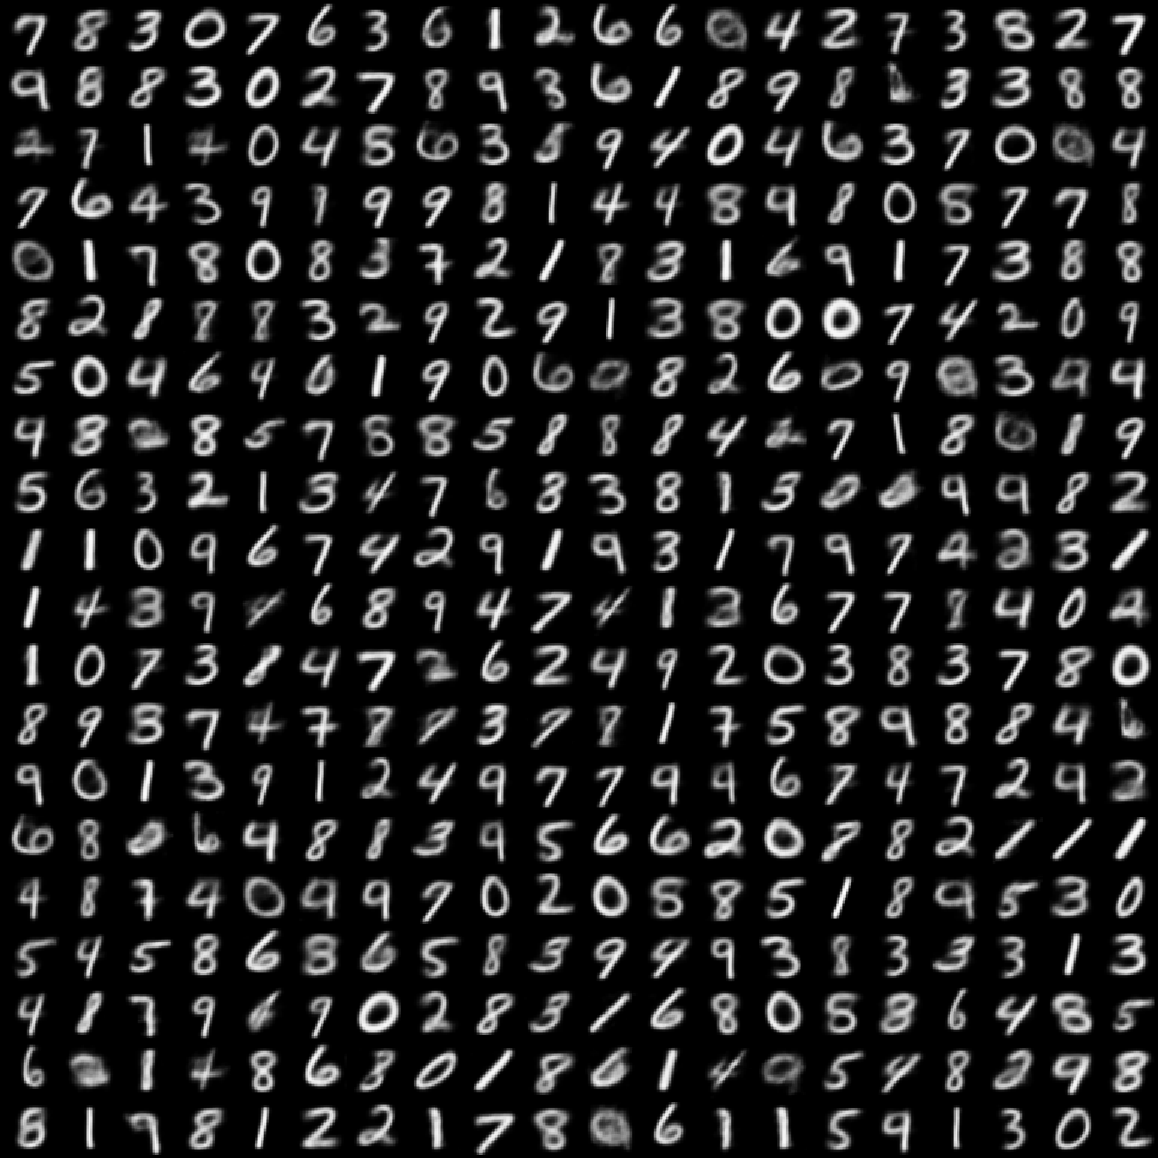
\includegraphics[width=0.8\linewidth]{figures/vae_samples}\\
    Randomly sampled
  \end{center}
\end{minipage}
\vfill

\NewPage\headline{Results: Reconstructions}
  \begin{center}
    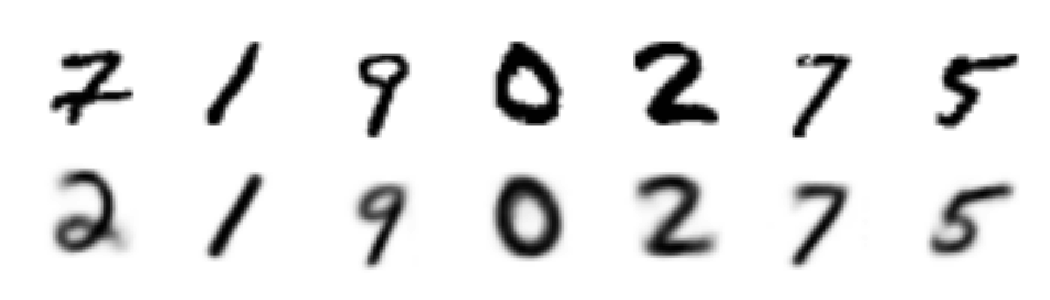
\includegraphics[width=\linewidth]{figures/reconstructions}\\
  \end{center}
  \vfill
  \begin{itemize}
    \item 50-dimensional latent space
    \item Used network architecture: 784-500-500-50
  \end{itemize}
\vfill



\NewPage\headline{Results: Learned Manifold}
  \begin{center}
    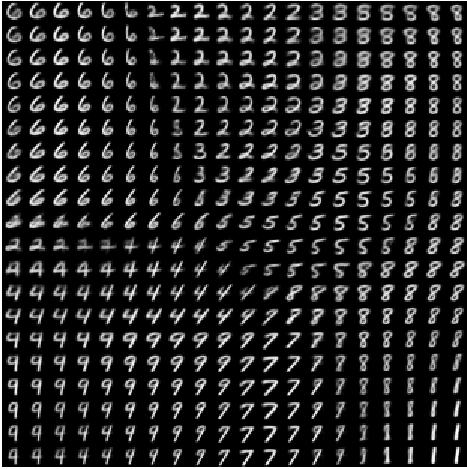
\includegraphics[width=0.5\linewidth]{figures/vae_manifold}\\
    Manifold plotting in 2-dimensional latent space $[-3,3]^2$
  \end{center}



%%%%%%%%%%%%%%%%%%%%%%%%%%%%%%%%%%%%%%%%%%%%%%%%%
\NewPage\headline{Generative Adversarial Nets}
\hypertarget{sli:gan}
\vfill
\begin{itemize}
  \item Proposed in 2014 by \cite{gan:2014}% Ian Goodfellow
  \item Simple game theoretic idea
  \item Two networks playing against each other:
  \begin{itemize}
    \item Generator $G$ tries to produce data like those in the dataset
    \item Discriminator $D$ tells fake and real data apart
  \end{itemize}
  \item Generator tries to fool the discriminator
  \item Hard to train
  %\item Has taken off in the last year (2016)
  %\item Simple idea, but hard to train
\end{itemize}
\vfill


\NewPage\headline{Generative Adversarial Nets}
  \begin{center}
    \includegraphics[width=\linewidth]{figures/gan_conceptual-crop}\\
  \end{center}


%%%%%%%%%%%%%%%%%%%%%%%%%%%%%%%%%%%%%%%%%%%%%%%%%
\NewPage\headline{More Directed Generative Models}
\hypertarget{sli:more}
\vfill
\begin{itemize}
  \item Helmholtz machine
  \item Generative moment matching networks
  \begin{itemize}
    \item Same idea as GANs
    \item Training using maximum mean discrepancy (MMD)
  \end{itemize}
  \item Auto-regressive networks
  \begin{itemize}
    \item Deep AutoRegressive Networks \cite{darn:2014}
    \begin{itemize}
      \item Deep generative autoencoder
    \end{itemize}
    \item PixelRNN \cite{pixelrnn:2016}
    \begin{itemize}
      \item model the conditional distribution of each pixel
    \end{itemize}
  \end{itemize}
\end{itemize}
\vfill


%%%%%%%%%%%%%%%%%%%%%%%%%%%%%%%%%%%%%%%%%%%%%%%%%
\NewPage\headline{Conclusion}
\hypertarget{sli:conclusion}
\vfill
\begin{itemize}
  \item Variational autoencoder
  \item Generative adversarial nets
  \begin{itemize}
    \item Good intuition with game-theoretic approach
  \end{itemize}
  \item Useful for high-dimensional real world data
  \begin{itemize}
    \item Build compact internal representation
  \end{itemize}
\end{itemize}
\vfill


%%%%%%%%%%%%%%%%%%%%%%%%%%%%%%%%%%%%%%%%%%%%%%%%%
\NewPage{References}
\bibliographystyle{i6bibliostyle}
\bibliography{presentation}


%%%%%%%%%%%%%%%%%%%%%%%%%%%%%%%%%%%%%%%%%%%%%%%%%
\FinalPage

\appendix
%%%%%%%%%%%%%%%%%%%%%%%%%%%%%%%%%%%%%%%%%%%%%%%%%%%%%%%%%%%%%%%%%%%%%%%%%%%%%%%%

\NewPage\headline{\appendixname: Model for Experiments}
\vfill
\begin{itemize}
  \item \textbf{Inference network}: 784 - 500 - 500 - z
  \item \textbf{Generative network}: z - 500 - 500 - 784
  \item Learning rate: $10^{-3}$
  \item Xavier initialization
  \item Rectifier linear units (ReLU)
  \item Sigmoid function for output layer
\end{itemize}
\vfill

\NewPage\headline{\appendixname: More Results (2-dim latent space)}
\begin{minipage}[t]{.5\linewidth}
  \begin{center}
    \includegraphics[height=8cm]{figures/mnist_samples_close_10dim.pdf}\\
    MNIST samples
  \end{center}
\end{minipage}
\begin{minipage}[t]{.5\linewidth}
  \begin{center}
    \includegraphics[height=8cm]{figures/vae_samples_close_2dim.pdf}
    VAE-generated samples with 10-dimensional $z$-space
  \end{center}
\end{minipage}

  \begin{center}
    \includegraphics{figures/reconstructions_2dim}\\
    Reconstructions using VAE in 10-dimensional $z$-space
  \end{center}

\NewPage\headline{\appendixname: More Results (10-dim latent space)}
\begin{minipage}[t]{.5\linewidth}
  \begin{center}
    \includegraphics[height=8cm]{figures/mnist_samples_close_10dim.pdf}\\
    MNIST samples
  \end{center}
\end{minipage}
\begin{minipage}[t]{.5\linewidth}
  \begin{center}
    \includegraphics[height=8cm]{figures/vae_samples_close_10dim.pdf}
    VAE-generated samples with 10-dimensional $z$-space
  \end{center}
\end{minipage}

  \begin{center}
    \includegraphics{figures/reconstructions_10dim}\\
    Reconstructions using VAE in 10-dimensional $z$-space
  \end{center}


\end{document}
